\section*{Appendix}

\subsection*{Site split formulation}
We begin by introducing ``site splits.''
We use site splits to formalize the notion that a given site pattern is equally probable to its complement under the binary symmetric model.
This is a standard step in the description of the Hadamard transform (Section 8.6 of \citet{Semple2003-em}), although our approach is complicated slightly by the inclusion of ancestral states.

Since we have a finite character alphabet, for a given column $i$ there are a finite number of possible assignments of characters to tips $\alignmentColumn_i$ or internal nodes $\ancestralStateColumn_i$.
For the binary symmetric model, the alphabet $\alphabet$ is $\{0,1\}$.
Take the tip labels of $\tau$ to be $\{1,\ldots,\nSiteRows\}$.
For likelihood calculation under the binary symmetric model, we describe a given $\alignmentColumn_i$ as a subset of indices $\siteSplit\subseteq\siteSplitSet:=\{1,\ldots,\nSiteRows-1\}$, commonly called a ``site split.''
Define the complement of $\alignmentColumn$ as $\overline{\alignmentColumn}$, and let $\alignmentColumn_{i,k}$ be the label of the $k$th tip in the $i$th alignment column.
We define the site split $\siteSplit$ for a $\alignmentColumn_i$ as the set of tips labeled with $1$ in $\alignmentColumn_i$ if the $\nSiteRows$th tip is not labeled with $1$, and as the set of tips labeled with $1$ in $\overline{\alignmentColumn}_i$ if the $\nSiteRows$th tip is labeled with $1$.
Taking such a complement simplifies but does not change the result of likelihood computation because the probability of observing a particular collection of binary characters is equivalent to the probability of its complement under the binary symmetric model.

For a fixed topology $\tau$, we define an ordered set of internal node labels $\{1,\ldots,\nAncestralStateRows\}$ for $\ancestralStateColumn_i$ and similarly use a subset of characters $\ancestralSplit\subseteq\ancestralSplitSet:=\{1,\ldots,\nAncestralStateRows\}$ to describe a realization $\ancestralStateColumn_i$.
In this case we cannot use the same complement trick as before: the probability of observing an ancestral state split conditional on a site split is not invariant to taking its complement.
We thus define an ``ancestral state split'' $\ancestralSplit$ for an internal node $\ancestralStateColumn_i$ to be the set of internal nodes labeled with $1$ if the $\nSiteRows$th tip is not labeled with $1$, and as the set of internal nodes labeled with $1$ in $\overline{\ancestralStateColumn}_i$ if the $\nSiteRows$th tip is labeled with $1$.
We emphasize that the ancestral state split complementing procedure depends on tip states, not ancestral states: both site splits and ancestral state splits are defined by whether the $\nSiteRows$th element of $\alignmentColumn_i$ is labeled as $1$.

We enumerate the site splits $\siteSplit_j$ of which there are $\nSiteSplits=|\mathcal{P}(\siteSplitSet)|$ in total where $\mathcal{P}$ denotes the power set.
Similarly we enumerate ancestral state splits $\ancestralSplit_k$ of which there are $\nAncestralSplits=|\mathcal{P}(\ancestralSplitSet)|$ in total.

We first fix notation.
\begin{definition}
Let the mapping from site patterns to site splits
\[
\patternToSplit:\alphabet^\nSiteRows\rightarrow\mathcal{P}(\siteSplitSet)
\]
be
\[
\patternToSplit(\alignmentColumn) =
\left\{
    \begin{array}{ll}
        \{i'\in\{1,\ldots,\nSiteRows-1\}: \alignmentColumn_{i,i'}=1\}  & \mbox{if } \alignmentColumn_{i,\nSiteRows}=0,\\
        \{i'\in\{1,\ldots,\nSiteRows-1\}: \overline{\alignmentColumn}_{i,i'}=1\}  & \mbox{if } \alignmentColumn_{i,\nSiteRows}=1,
    \end{array}
\right.
\]
and the mapping from ancestral states and tip states to ancestral state splits
\[
\ancestralToSplit:\alphabet^\nSiteRows\times\alphabet^\nAncestralStateRows\rightarrow\mathcal{P}(\ancestralSplitSet)
\]
be
\[
\ancestralToSplit(\alignmentColumn, \ancestralStateColumn) =
\left\{
    \begin{array}{ll}
        \{i'\in\{1,\ldots,\nAncestralStateRows\}: \ancestralStateColumn_{i,i'}=1\}  & \mbox{if } \alignmentColumn_{i,\nSiteRows}=0,\\
        \{i'\in\{1,\ldots,\nAncestralStateRows\}: \overline{\ancestralStateColumn}_{i,i'}=1\}  & \mbox{if } \alignmentColumn_{i,\nSiteRows}=1.
    \end{array}
\right.
\]
Then, given a site pattern--valued random variable $\alignmentColumnRV$ and an ancestral state--valued random variable $\ancestralStateColumnRV$, define the random variables
\[
\siteSplitRV := \patternToSplit(\alignmentColumnRV)
\]
and
\[
\ancestralSplitRV := \ancestralToSplit(\alignmentColumnRV, \ancestralStateColumnRV).
\]
\end{definition}
The mapping $\patternToSplit$ operates by returning the tips labeled as $1$ in a site pattern to obtain a site split in $\mathcal{P}(\siteSplitSet)$ if the set of tips labeled $1$ is not in $\mathcal{P}(\siteSplitSet)$.
The mapping $\ancestralToSplit$ is defined by whether the tip states have their complements taken or not: if the set of tips labeled $1$ in $\alignmentColumn$ is in $\mathcal{P}(\siteSplitSet)$, $\ancestralToSplit(\alignmentColumn, \ancestralStateColumn)$ is the set of tips labeled $1$ in $\ancestralStateColumn$; otherwise, the set of tips labeled $1$ in $\overline{\alignmentColumn}$ necessarily is in $\mathcal{P}(\siteSplitSet)$ and so $\ancestralToSplit(\alignmentColumn, \ancestralStateColumn)$ is $\overline{\ancestralStateColumn}$.

We now consider the $i$th factor of \eqref{eq:full_likelihood}.
As a consequence of assuming a binary symmetric model, for some $\siteSplit_j\in\mathcal{P}(\siteSplitSet)$ the mapping $\patternToSplit(\alignmentColumn_i)$ has the property
\begin{align*}
    \Pr(\siteSplitRV=\siteSplit_j, \ancestralSplitRV=\ancestralSplit_k \mid \tau, t) &= \Pr(\siteSplitRV=\patternToSplit(\alignmentColumn_i), \ancestralSplitRV=\ancestralToSplit(\alignmentColumn_i, \ancestralStateColumn_i) \mid \tau, t)\\
    &= \Pr((\alignmentColumnRV=\alignmentColumn_i, \ancestralStateColumnRV=\ancestralStateColumn_i) \cup (\overline{\alignmentColumnRV}=\alignmentColumn_i, \overline{\ancestralStateColumnRV}=\ancestralStateColumn_i) \mid \tau, t)\\
    &= \Pr(\alignmentColumnRV=\alignmentColumn_i, \ancestralStateColumnRV=\ancestralStateColumn_i \mid \tau, t) + \Pr(\overline{\alignmentColumnRV}=\alignmentColumn_i, \overline{\ancestralStateColumnRV}=\ancestralStateColumn_i \mid \tau, t)\\
    &= 2\cdot\Pr(\alignmentColumnRV=\alignmentColumn_i, \ancestralStateColumnRV=\ancestralStateColumn_i \mid \tau, t)
\end{align*}
where $\overline{\alignmentColumnRV}$ is the complement of the site pattern--valued random variable $\alignmentColumnRV$ and has the same distribution as $\alignmentColumnRV$ (similarly for $\ancestralStateColumnRV$).
Since
\begin{align*}
    2\cdot\Pr(\alignmentColumnRV=\alignmentColumn_i, \ancestralStateColumnRV=\ancestralStateColumn_i \mid \tau, t) &= \Pr(\siteSplitRV=\patternToSplit(\alignmentColumn_i), \ancestralSplitRV=\ancestralToSplit(\alignmentColumn_i, \ancestralStateColumn_i) \mid \tau, t),
\end{align*}
given $(\tau, t)$, there exist sets $\ancestralSplitPartition_1(\tau, t),\ldots,\ancestralSplitPartition_\nSiteSplits(\tau, t)$ such that $\xi_{\siteSplit_j}\in\ancestralSplitPartition_j(\tau, t)$ satisfies
\begin{align*}
\max_{\ancestralSplit_k\in\mathcal{P}(\ancestralSplitSet)} \ \Pr(\siteSplitRV=\siteSplit_j, \ancestralSplitRV=\ancestralSplit_k \mid \tau, t) &= \Pr(\siteSplitRV=\siteSplit_j, \ancestralSplitRV = \xi_{\siteSplit_j} \mid \tau, t).
\end{align*}
In other words, for the $j$th site split, $\ancestralSplitPartition_j(\tau, t)\subseteq\mathcal{P}(\ancestralSplitSet)$ is the set of most likely ancestral state splits for that particular site split, topology and set of branch lengths, i.e., $\ancestralSplitPartition_j(\tau, t)$ is a set of sets of most likely internal node labels.
Here, $\xi_{\siteSplit_j}$ is one of possibly many equiprobable ancestral state splits in $\ancestralSplitPartition_j(\tau, t)$.
For each $\alignmentColumn_i$, $\ancestralToSplit(\alignmentColumn_i, \cdot)$ is surjective as it can map values from $\alphabet^\nAncestralStateRows$ to all elements in $\mathcal{P}(\ancestralSplitSet)$.
This can be seen by using the definition of $\ancestralToSplit(\alignmentColumn_i, \cdot)$ and assuming $\alignmentColumn_{i,\nSiteRows}=0$, where in this case each of the $2^\nAncestralStateRows$ values of $\ancestralStateColumn$ correspond to each of the $2^\nAncestralStateRows$ elements of $\mathcal{P}(\{1,\ldots,\nAncestralStateRows\})$.
The same can be done for the case of $\alignmentColumn_{i,\nSiteRows}=1$, implying $\ancestralToSplit(\alignmentColumn_i, \cdot)$ is surjective.
From this we have
\begin{align*}
    \max_{\ancestralStateColumn_i} \ 2\cdot\Pr(\alignmentColumnRV=\alignmentColumn_i, \ancestralStateColumnRV=\ancestralStateColumn_i \mid \tau, t) &= \max_{\ancestralStateColumn_i} \ \Pr(\siteSplitRV=\patternToSplit(\alignmentColumn_i), \ancestralSplitRV=\ancestralToSplit(\alignmentColumn_i, \ancestralStateColumn_i) \mid \tau, t)\\
    &= \max_{\ancestralSplit_k\in\mathcal{P}(\ancestralSplitSet)} \ \Pr(\siteSplitRV=\siteSplit_j, \ancestralSplitRV=\ancestralSplit_k \mid \tau, t)\\
    &= \Pr(\siteSplitRV=\siteSplit_j, \ancestralSplitRV = \xi_{\siteSplit_j} \mid \tau, t)
\end{align*}
for some $j$.
Thus, each term in the likelihood can be collapsed into terms relating only to site splits and ancestral state splits, indexed by $j$, as opposed to individual observations, indexed by $i$.

\subsection*{Example}
We follow with an example computing these probabilities and likelihoods.
Consider the fixed, binary four-taxon tree $\tau_1$ in Fig.~\ref{fig:farris-fels-top}a.
The set of all possible character assignments is
\begin{align*}
\mathcal{P}(\{1,2,3,4\}) &= \{\emptyset, \{1,2,3,4\}, \{1\}, \{2,3,4\}, \{2\}, \{1,3,4\}, \{3\}, \{1,2,4\}, \\
                         &\qquad \{1,2\}, \{3,4\}, \{1,3\}, \{2,4\}, \{2,3\}, \{1,4\}, \{1,2,3\}, \{1,4\}\}
\end{align*}
where each set indicates the tips assigned the character $1$.
For example, $\emptyset$ is the labeling $0000$ and $\{1,3,4\}$ is the labeling $1011$.
Symmetry allows us to group adjacent pairs in $\mathcal{P}(\{1,2,3,4\})$ into equiprobable splits, letting $\siteSplitSet=\{1,2,3\}$.
The unique site splits, collapsing complements, are
\begin{align*}
    \mathcal{P}(\siteSplitSet) &= \{\emptyset, \{1\}, \{2\}, \{3\}, \{1,2\}, \{1,3\}, \{2,3\}, \{1,2,3\}\} \\
& =: \{\siteSplit_1, \ldots, \siteSplit_8\}.
\end{align*}
Since we identify character complements, we do not consider the additional splits
\begin{equation*}
\begin{split}
& \mathcal{P}(\{1,2,3,4\}) \setminus \mathcal{P}(\siteSplitSet) = \\
&\qquad \{\{1,2,3,4\}, \{2,3,4\}, \{1,3,4\}, \{1,2,4\}, \{3,4\}, \{2,4\}, \{1,4\}, \{4\}\},
\end{split}
\end{equation*}
the symmetry of the binary character model allowing us to focus only on the elements of $\mathcal{P}(\siteSplitSet)$.
This tree has two internal nodes with $\ancestralSplitSet=\{1,2\}$ and unique ancestral state splits
\[
\mathcal{P}(\ancestralSplitSet) = \{\emptyset, \{1\}, \{2\}, \{1,2\}\}.
\]
Internal node $1$ is the node connected to leaves $1$ and $3$ while internal node $2$ is connected to leaves $2$ and $4$.
The mapping from characters to splits in this case depends on the characters at the tips and the ancestral states.
For example, we take both $\patternToSplit(0000)=\emptyset$ and $\patternToSplit(1111)=\emptyset$.
Similarly, we have $\ancestralToSplit(0000, 00) = \emptyset$ and $\ancestralToSplit(1111, 11)=\emptyset$, needing to take the complement of all the characters present on the tree to identify splits.
We cannot identify complements for ancestral states in the same way as tip states since, for $\siteSplit\in\mathcal{P}(\siteSplitSet)$,
\[
\Pr(\siteSplitRV=\siteSplit, \ancestralSplitRV=\emptyset \mid \tau, t)\neq \Pr(\siteSplitRV=\siteSplit, \ancestralSplitRV=\{1,2\} \mid \tau, t)
\]
in general.

For each site split $\siteSplit\in\mathcal{P}(\siteSplitSet)$, we maximize the likelihood over all $\ancestralSplit\in\mathcal{P}(\ancestralSplitSet)$.
A maximum occurs at one of possibly several ancestral state splits in $\mathcal{P}(\ancestralSplitSet)$, defined via $\ancestralSplitPartition_j(\tau, t)$ for the $j$th site split.
As a simple example, say all branch lengths correspond to a probability $p$ ($< 1/2$) of changing character along that branch, with $t=\{p,p,p,p,p\}$.
The probabilities of observing ancestral state splits for $\siteSplit_1=\emptyset$ are
\[
\Pr(\siteSplitRV=\emptyset, \ancestralSplitRV=\emptyset \mid \tau, t) =
(1-p)^5,
\]
\[
\Pr(\siteSplitRV=\emptyset, \ancestralSplitRV=\{1\} \mid \tau, t) =
\Pr(\siteSplitRV=\emptyset, \ancestralSplitRV=\{2\} \mid \tau, t) =
p^3(1-p)^2,
\]
\[
\Pr(\siteSplitRV=\emptyset, \ancestralSplitRV=\{1,2\} \mid \tau, t) =
p^4(1-p).
\]
The set of most likely ancestral states contains a single element, here $\ancestralSplitPartition_1(\tau, t)=\{\emptyset\}$.
Then, taking $\xi_{\emptyset}\in\ancestralSplitPartition_1(\tau, t)$ we have
\[
\Pr(\siteSplitRV=\emptyset, \ancestralSplitRV=\xi_{\emptyset} \mid \tau, t) =
\Pr(\siteSplitRV=\emptyset, \ancestralSplitRV=\emptyset \mid \tau, t) =
(1-p)^5.
\]
For $\siteSplit_5=\{1,2\}$ we have
\[
\Pr(\siteSplitRV=\{1,2\}, \ancestralSplitRV=\emptyset \mid \tau, t) =
\Pr(\siteSplitRV=\{1,2\}, \ancestralSplitRV=\{1,2\} \mid \tau, t) =
p^2(1-p)^3,
\]
\[
\Pr(\siteSplitRV=\{1,2\}, \ancestralSplitRV=\{1\} \mid \tau, t) =
\Pr(\siteSplitRV=\{1,2\}, \ancestralSplitRV=\{2\} \mid \tau, t) =
p^3(1-p)^2.
\]
Here, the set of most likely ancestral states is $\ancestralSplitPartition_5(\tau, t)=\{\emptyset,\{1,2\}\}$, and, for $\xi_{12}\in\ancestralSplitPartition_5(\tau, t)$,
\[
\Pr(\siteSplitRV=\{1,2\}, \ancestralSplitRV=\xi_{12} \mid \tau, t) =
p^2(1-p)^3.
\]

\subsection*{Site split likelihood}

The likelihood in \eqref{eq:profile_likelihood} can be written as
\begin{align}
L_\nCols'(\tau, t; \fullAlignment) &= \max_{\fullAncestralStates} \ L_\nCols(\tau, t; \fullAlignment, \fullAncestralStates) \nonumber \\
                             &= \prod_{i=1}^{\nCols} \ \max_{\ancestralStateColumn_i} \ \Pr(\alignmentColumnRV=\alignmentColumn_i, \ancestralStateColumnRV=\ancestralStateColumn_i \mid \tau, t) \nonumber \\
                             &\propto \prod_{i=1}^{\nCols} \ \max_{\ancestralStateColumn_i} \ \Pr(\siteSplitRV=\patternToSplit(\alignmentColumn_i), \ancestralSplitRV=\ancestralToSplit(\alignmentColumn_i, \ancestralStateColumn_i) \mid \tau, t) \nonumber \\
                             &= \prod_{i=1}^{\nCols} \ \Pr(\siteSplitRV=\siteSplit_j, \ancestralSplitRV=\xi_{\siteSplit_j} \mid \tau, t) \nonumber \\
                             &= \prod_{j=1}^{\nSiteSplits} \ \left[\Pr(\siteSplitRV=\siteSplit_j, \ancestralSplitRV=\xi_{\siteSplit_j} \mid \tau, t)\right] ^{\nCols_j(\fullAlignment)} \label{eq:site_pattern_likelihood}
\end{align}
for $\siteSplit_j\in\mathcal{P}(\siteSplitSet)$ and some $\xi_{\siteSplit_j}\in\ancestralSplitPartition_j(\tau, t)$ with $1 \le j \le q$ where $\nCols_j(\fullAlignment)$ is the number of columns in $\fullAlignment$ that project to site split $\siteSplit_j$.

Let
\[
L_\nCols''(\tau, t; \fullAlignment) = \prod_{j=1}^{\nSiteSplits} \ \left[\Pr(\siteSplitRV=\siteSplit_j, \ancestralSplitRV=\xi_{\siteSplit_j} \mid \tau, t)\right] ^{\nCols_j(\fullAlignment)}
\]
be the final product in \eqref{eq:site_pattern_likelihood}.
Assume $\nCols$ observations are generated from a model with parameters $(\tau^*, t^*)$.
We have
\begin{equation*}
\frac{1}{\nCols} \log L_\nCols''(\tau, t; \fullAlignment) = \sum_{j=1}^\nSiteSplits \frac{\nCols_j(\fullAlignment)}{\nCols}\cdot  \log \Pr(\siteSplitRV=\siteSplit_j, \ancestralSplitRV=\xi_{\siteSplit_j} \mid \tau, t)
\end{equation*}
so that, in the $\nCols\rightarrow\infty$ limit,
\begin{equation}
\begin{split}
&    \frac{1}{\nCols} \log L_\nCols''(\tau, t; \fullAlignment) \\
&\qquad \rightarrow \sum_{j=1}^\nSiteSplits \Pr(\siteSplitRV=\siteSplit_j \mid \tau^*, t^*) \cdot \log \Pr(\siteSplitRV=\siteSplit_j, \ancestralSplitRV=\xi_{\siteSplit_j} \mid \tau, t). \label{eq:site_pattern_profile_likelihood_mean}
\end{split}
\end{equation}

\subsection*{Hadamard representation}

We state the Hadamard representation of site split generating probabilities---that is, probabilities of obtaining particular site splits given a tree---following Section 8.6 of \citet{Semple2003-em}.
For each edge $e$ define the edge ``fidelity'' for that edge as
\[
\theta(e) = 1-2p(e)
\]
where $p(e)$ is the probability of a character change along edge $e$.
For an even-sized subset of $Y\subseteq\mathcal{S}$, let the path set $P(Y)$ be the set of edges in the path connecting both elements of $Y$.
For $n$ taxa, the probability of observing site split $A\in\mathcal{P}(\siteSplitSet)$ is
\begin{equation}
\label{eq:hadamard_probability}
p_A = \frac{1}{2^{n-1}} \ \sum_{Y \subseteq \mathcal{S} : |Y| \equiv 0 (\mathrm{mod} \ 2)} \ \left[(-1)^{|Y \cap A|} \ \prod_{e\in P(Y)} \ \theta(e) \right].
\end{equation}
By convention, we set $P(\emptyset)=\emptyset$ and $\prod_{e\in\emptyset} \ \theta(e) = 1$.
For notational convenience, let
\[
p_{\siteSplit_j} := \Pr(\siteSplitRV=\siteSplit_j \mid \tau_1,t),
\]
for any site split $\siteSplit_j$.
Table~\ref{tab:gen-sitepatprob} contains calculations of site split probabilities for the trees in Fig.~\ref{fig:farris-fels-top}.

\begin{table}[ht]
\centering
\begin{tabular}{|l|l|l|}
    \multicolumn{3}{c}{InvFels tree $\tau=\tau^*$, $t^*=\{x^*,y^*,x^*,y^*,y^*\}$}\\
    \hline
$\siteSplit_j$  & $p_{\siteSplit_j}$ &$8\cdot\Pr(\siteSplitRV=\siteSplit_j \mid \tau,t)$\\
    \hline
    $\emptyset$ & $p_{\emptyset}$   &$1+(x^*)^2+(y^*)^2+4x^*(y^*)^2+(x^*)^2(y^*)^2$\\
    $\{1\}$     & $p_{1}$           &$1-(x^*)^2+(y^*)^2-(x^*)^2(y^*)^2$\\
    $\{2\}$     & $p_{2}$           &$1+(x^*)^2-(y^*)^2-(x^*)^2(y^*)^2$\\
    $\{3\}$     & $p_{3}$           &$1-(x^*)^2+(y^*)^2-(x^*)^2(y^*)^2$\\
    $\{1,2,3\}$ & $p_{123}$         &$1+(x^*)^2-(y^*)^2-(x^*)^2(y^*)^2$\\
    $\{1,2\}$   & $p_{12}$          &$1-(x^*)^2-(y^*)^2+(x^*)^2(y^*)^2$\\
    $\{2,3\}$   & $p_{23}$          &$1-(x^*)^2-(y^*)^2+(x^*)^2(y^*)^2$\\
    $\{1,3\}$   & $p_{13}$          &$1+(x^*)^2+(y^*)^2-4x^*(y^*)^2+(x^*)^2(y^*)^2$\\
    \hline
    \multicolumn{3}{c}{InvFels tree $\tau=\tau_1$, $t=\{x_1,y_1,x_2,y_2,w\}$}\\
    \hline
$\siteSplit_j$  & $p_{\siteSplit_j}$ &$8\cdot\Pr(\siteSplitRV=\siteSplit_j \mid \tau,t)$\\
    \hline
    $\emptyset$ & $p_{\emptyset}$   &$1 + x_1x_2 +  y_1y_2 +  w[  x_1 + x_2][  y_1 + y_2] + x_1y_1x_2y_2$\\
    $\{1\}$     & $p_{1}$           &$1 - x_1x_2 +  y_1y_2 +  w[- x_1 + x_2][  y_1 + y_2] - x_1y_1x_2y_2$\\
    $\{2\}$     & $p_{2}$           &$1 + x_1x_2 -  y_1y_2 +  w[  x_1 + x_2][- y_1 + y_2] - x_1y_1x_2y_2$\\
    $\{3\}$     & $p_{3}$           &$1 - x_1x_2 +  y_1y_2 +  w[  x_1 - x_2][  y_1 + y_2] - x_1y_1x_2y_2$\\
    $\{1,2,3\}$ & $p_{123}$         &$1 + x_1x_2 -  y_1y_2 +  w[  x_1 + x_2][  y_1 - y_2] - x_1y_1x_2y_2$\\
    $\{1,2\}$   & $p_{12}$          &$1 - x_1x_2 -  y_1y_2 +  w[- x_1 + x_2][- y_1 + y_2] + x_1y_1x_2y_2$\\
    $\{2,3\}$   & $p_{23}$          &$1 - x_1x_2 -  y_1y_2 +  w[  x_1 - x_2][- y_1 + y_2] + x_1y_1x_2y_2$\\
    $\{1,3\}$   & $p_{13}$          &$1 + x_1x_2 +  y_1y_2 +  w[- x_1 - x_2][  y_1 + y_2] + x_1y_1x_2y_2$\\
    \hline
    \multicolumn{3}{c}{Felsenstein tree $\tau=\tau_2$, $t=\{x_1,y_1,x_2,y_2,w\}$}\\
    \hline
$\siteSplit_j$  & $p_{\siteSplit_j}$ &$8\cdot\Pr(\siteSplitRV=\siteSplit_j \mid \tau,t)$\\
    \hline
    $\emptyset$ & $p_{\emptyset}$   &$1 + x_1y_1 +  x_2y_2 +  w[  x_1 + y_1][  x_2 + y_2] + x_1y_1x_2y_2$\\
    $\{1\}$     & $p_{1}$           &$1 - x_1y_1 +  x_2y_2 +  w[ -x_1 + y_1][  x_2 + y_2] - x_1y_1x_2y_2$\\
    $\{2\}$     & $p_{2}$           &$1 - x_1y_1 +  x_2y_2 +  w[  x_1 - y_1][  x_2 + y_2] - x_1y_1x_2y_2$\\
    $\{3\}$     & $p_{3}$           &$1 + x_1y_1 -  x_2y_2 +  w[  x_1 + y_1][ -x_2 + y_2] - x_1y_1x_2y_2$\\
    $\{1,2,3\}$ & $p_{123}$         &$1 + x_1y_1 -  x_2y_2 +  w[ -x_1 - y_1][ -x_2 + y_2] - x_1y_1x_2y_2$\\
    $\{1,2\}$   & $p_{12}$          &$1 + x_1y_1 +  x_2y_2 +  w[ -x_1 - y_1][  x_2 + y_2] + x_1y_1x_2y_2$\\
    $\{2,3\}$   & $p_{23}$          &$1 - x_1y_1 -  x_2y_2 +  w[  x_1 - y_1][ -x_2 + y_2] + x_1y_1x_2y_2$\\
    $\{1,3\}$   & $p_{13}$          &$1 - x_1y_1 -  x_2y_2 +  w[ -x_1 + y_1][ -x_2 + y_2] + x_1y_1x_2y_2$\\
    \hline
\end{tabular}
\caption{8 times the site split probabilities $p_{\siteSplit_j}$ on the true InvFels tree $\tau^*$ with $t^*=\{x^*,y^*,x^*,y^*,y^*\}$, and on the InvFels tree $\tau_1$ and Felsenstein tree $\tau_2$ with $t=\{x_1,y_1,x_2,y_2,w\}$ obtained using the Hadamard transform.
}
\label{tab:gen-sitepatprob}
\end{table}

\subsection*{Likelihood computations}

To compute the likelihood of observing a set of data, we need $\Pr(\siteSplitRV=\siteSplit_j, \ancestralSplitRV=\ancestralSplit_k \mid \tau, t)$ for each $\ancestralSplit_k$ and $\siteSplit_j$.
Using branch fidelities, the probability of a character change along a branch with fidelity parameter $x$ is $(1-x)/2$, while the probability of a character remaining the same is $(1+x)/2$.
See Fig.~\ref{fig:example_likelihoods} for the parameters on an example site pattern on the InvFels tree.
Likelihood computations for all site splits and ancestral state splits are in Table~\ref{tab:farris_likelihoods} for the InvFels tree.

\begin{figure}
\centering
\begin{subfigure}{.45\linewidth}
\centering
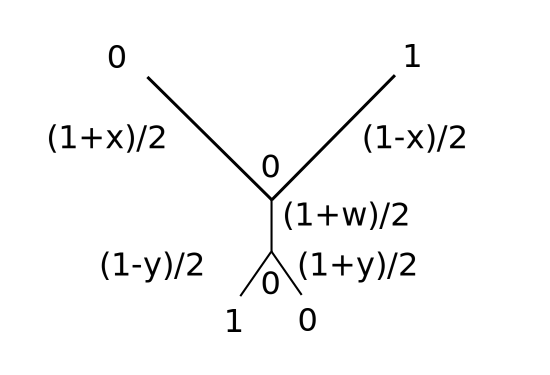
\includegraphics[width=.95\textwidth]{farris_like00}
\caption[short]{}
\end{subfigure}
\begin{subfigure}{.45\linewidth}
\centering
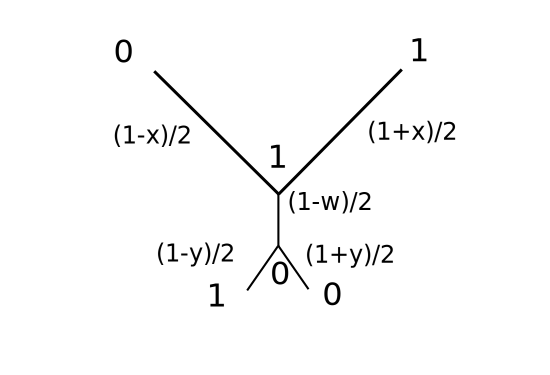
\includegraphics[width=.95\textwidth]{farris_like10}
\caption[short]{}
\end{subfigure}
\caption{
    Example likelihood computations on the InvFels tree $\tau_1$ for fidelities $t=\{x_1,y_1,x_2,y_2,w\}$.
    Edges labeled by the probability of substitution along that edge.
    In (a), we compute the product to obtain $\Pr(\siteSplitRV=\{2,3\},\ancestralSplitRV=\emptyset\mid \tau_1,t) = (1+x_1)(1-x_2)(1+y_1)(1-y_2)(1+w)/32$.
    In (b), the same process yields $\Pr(\siteSplitRV=\{2,3\},\ancestralSplitRV=\{1\}\mid \tau_1,t) = (1+x_1)(1-x_2)(1+y_1)(1-y_2)(1-w)/32$.
}
\label{fig:example_likelihoods}
\end{figure}

\begin{table}
\centering
\begin{tabular}{|l|ll|}
\hline
$\siteSplit_j$ & $\ancestralSplit_k$ & $32\cdot\Pr(\siteSplitRV=\siteSplit_j, \ancestralSplitRV=\ancestralSplit_k \mid \tau_1, t)$\\
\hline
$\emptyset$&$\emptyset$&$(1+x_1)(1+y_1)(1+x_2)(1+y_2)(1+w)$\\
&$\{1\}^*$&$(1-x_1)(1+y_1)(1-x_2)(1+y_2)(1-w)$             \\
&$\{2\}^*$&$(1+x_1)(1-y_1)(1+x_2)(1-y_2)(1-w)$             \\
&$\{1,2\}^*$&$(1-x_1)(1-y_1)(1-x_2)(1-y_2)(1+w)$           \\

$\{1\}$    &$\emptyset$&$(1-x_1)(1+y_1)(1+x_2)(1+y_2)(1+w)$\\
&$\{1\}$&$(1+x_1)(1+y_1)(1-x_2)(1+y_2)(1-w)$               \\
&$\{2\}^*$&$(1-x_1)(1-y_1)(1+x_2)(1-y_2)(1-w)$             \\
&$\{1,2\}$&$(1+x_1)(1-y_1)(1-x_2)(1-y_2)(1+w)$             \\

$\{2\}$    &$\emptyset$&$(1+x_1)(1-y_1)(1+x_2)(1+y_2)(1+w)$\\
&$\{1\}^*$&$(1-x_1)(1-y_1)(1-x_2)(1+y_2)(1-w)$             \\
&$\{2\}$&$(1+x_1)(1+y_1)(1+x_2)(1-y_2)(1-w)$               \\
&$\{1,2\}$&$(1-x_1)(1+y_1)(1-x_2)(1-y_2)(1+w)$             \\

$\{3\}$    &$\emptyset$&$(1+x_1)(1+y_1)(1-x_2)(1+y_2)(1+w)$\\
&$\{1\}$&$(1-x_1)(1+y_1)(1+x_2)(1+y_2)(1-w)$               \\
&$\{2\}^*$&$(1+x_1)(1-y_1)(1-x_2)(1-y_2)(1-w)$             \\
&$\{1,2\}$&$(1-x_1)(1-y_1)(1+x_2)(1-y_2)(1+w)$             \\

$\{1,2,3\}$&$\emptyset$&$(1-x_1)(1-y_1)(1-x_2)(1+y_2)(1+w)$\\
&$\{1\}$&$(1+x_1)(1-y_1)(1+x_2)(1+y_2)(1-w)$               \\
&$\{2\}^*$&$(1-x_1)(1+y_1)(1-x_2)(1-y_2)(1-w)$             \\
&$\{1,2\}$&$(1+x_1)(1+y_1)(1+x_2)(1-y_2)(1+w)$             \\

$\{1,2\}$  &$\emptyset$&$(1-x_1)(1-y_1)(1+x_2)(1+y_2)(1+w)$\\
&$\{1\}$&$(1+x_1)(1-y_1)(1-x_2)(1+y_2)(1-w)$               \\
&$\{2\}$&$(1-x_1)(1+y_1)(1+x_2)(1-y_2)(1-w)$               \\
&$\{1,2\}$&$(1+x_1)(1+y_1)(1-x_2)(1-y_2)(1+w)$             \\

$\{2,3\}$  &$\emptyset$&$(1+x_1)(1-y_1)(1-x_2)(1+y_2)(1+w)$\\
&$\{1\}$&$(1-x_1)(1-y_1)(1+x_2)(1+y_2)(1-w)$               \\
&$\{2\}$&$(1+x_1)(1+y_1)(1-x_2)(1-y_2)(1-w)$               \\
&$\{1,2\}$&$(1-x_1)(1+y_1)(1+x_2)(1-y_2)(1+w)$             \\

$\{1,3\}$  &$\emptyset$&$(1-x_1)(1+y_1)(1-x_2)(1+y_2)(1+w)$\\
&$\{1\}$&$(1+x_1)(1+y_1)(1+x_2)(1+y_2)(1-w)$               \\
&$\{2\}^*$&$(1-x_1)(1-y_1)(1-x_2)(1-y_2)(1-w)$             \\
&$\{1,2\}$&$(1+x_1)(1-y_1)(1+x_2)(1-y_2)(1+w)$             \\
\hline
\end{tabular}
\caption{
32 times likelihood values for all site splits $\siteSplit_j$ and ancestral state splits $\ancestralSplit_k$ of the InvFels tree $\tau_1$.
Ancestral states with $^*$ are never maximal provided parameters are in $(0,1]$.
By combinations of $\ancestralSplit_k$, there are $3^5\cdot 4^2=3,888$ possible forms for the likelihood.
}
\label{tab:farris_likelihoods}
\end{table}

%TODO: the caption of this overlaps with the page number---will this be a problem or will MBE handle it?
%EM There is a latex package for that, which I tried out and then removed for some reason. It's no bigs.

\subsection*{Convergence of branch parameters}

%das: @EM I think this is actually the same Wald reference that Felsenstein tried to use.
%It works here for a fixed topology, and didn't work for him or your reference because I think the upper-semicontinuous condition doesn't hold for trees in general.
%Also I don't think the compactness condition holds---tree space isn't compact is it?
%However we now have a potential snag in that we are doing what Yang (1994) in his intro says is bad, i.e., doing ML for fixed, separate topologies and comparing them.
%We still have the behavior in the plots and the proofs, since they all assumed a fixed topology, and I think everything's fine with the arguments about Fels vs InvFels, but maybe you can let me know what you think?
For a fixed $\tau$, we show that $\hat{t}_\nCols \rightarrow \hat{t}$ for
\[
\hat{t}_\nCols = \arg\max_{t\in\mathcal{T}} \ \frac{1}{n}\log L_\nCols'(\tau, t; \fullAlignment)
\]
and
\[
\hat{t} = \arg\max_{t\in\mathcal{T}} \ \ell_{\tau^*,t^*}(\tau, t; \boldsymbol\xi).
\]
Using the notation in Section 5.2.1 in \citet{van1998asymptotic}, we let
\[
m_t(\alignmentColumn) = \sum_{j=1}^\nSiteSplits 1\{\patternToSplit(\alignmentColumn)=\siteSplit_j\} \cdot \log \Pr(\siteSplitRV=\siteSplit_j, \ancestralSplitRV=\xi_{\siteSplit_j} \mid \tau, t)
\]
so that
\[
\frac{1}{n}\log L_\nCols'(\tau, t; \fullAlignment) = \frac{1}{n} \sum_{i=1}^\nCols m_t(\alignmentColumn_i)
\]
and
\[
\ell_{\tau^*,t^*}(\tau, t; \boldsymbol\xi) = E[m_t].
\]
To show $\hat{t}_\nCols \rightarrow \hat{t}$, we use Wald's consistency proof \citep[p. 48, Theorem 5.14 of ][]{van1998asymptotic}, which requires four conditions.
The first is that $\mathcal{T}$ is compact, which is obviously true.
The second is that
\[
E\left[\sup_{t\in\mathcal{T}} m_t\right] < \infty,
\]
and, since $m_t(\alignmentColumn)$ is nonpositive for all $t$ and $\alignmentColumn$, this property holds.
The remaining conditions are on the maps
\[
\alignmentColumn \mapsto \sup_t m_t(\alignmentColumn)
\]
and
\[
t \mapsto m_t(\alignmentColumn).
\]
We need the first map to be measurable, which is evident since the domain $\alphabet^\nSiteRows$ of the mapping is a finite set, and so all subsets of the domain are also finite and thus measurable.
Finally, we must have the the second mapping be upper-semicontinuous for almost all $\alignmentColumn$.
For a fixed ancestral state split $t \mapsto m_t(\alignmentColumn)$ is continuous for all $\alignmentColumn$.
If we move about in $\mathcal{T}$, a different ancestral state split becomes more likely, though when we maximize over ancestral state splits we obtain a continuous function since the maximum over continuous functions is also continuous.
This ensures the upper-semicontinuous property of this mapping, and shows $\hat{t}_\nCols \rightarrow \hat{t}$, allowing our consistency results to be proved using $\ell_{\tau^*,t^*}(\tau, t; \boldsymbol\xi)$.

\subsection*{Properties of the joint objective function}

Consider the InvFels tree $\tau_1$ with arbitrary fidelities, i.e., $t=\{x_1,y_1,x_2,y_2,w\}$.
Next we show that the likelihood $\ell_{\tau_1,t}(\tau_1, t; \boldsymbol\xi)$ remains unchanged if $x_1$ and $x_2$ are exchanged or if $y_1$ and $y_2$ are.
Although this property should not be surprising due to symmetry, we write it out for completeness.
This holds for a general $t$, and thus holds setting $t=t^*$.
Using the Hadamard transform, we calculate the generating probabilities on the InvFels tree.
For site split $\emptyset$,
\begin{align*}
    \Pr(\siteSplitRV=\emptyset\mid \tau_1, t) & = \frac{1}{8} (1 + x_1x_2 +  y_1y_2 +  x_1y_1w + x_1y_2w + y_1x_2w + x_2y_2w + x_1y_1x_2y_2) \\
                                              & = \frac{1}{8} (1 + x_1x_2 +  y_1y_2 +  w[x_1y_1 + x_1y_2 + y_1x_2 + x_2y_2] + x_1y_1x_2y_2) \\
                                              & = \frac{1}{8} (1 + x_1x_2 +  y_1y_2 +  w[x_1 + x_2][y_1 + y_2] + x_1y_1x_2y_2),
\end{align*}
and this probability is unchanged when $x_1$ is exchanged with $x_2$ and $y_1$ is exchanged with $y_2$.
Similarly, for site split $\{1,3\}$,
\[
    \Pr(\siteSplitRV=\{1,3\}\mid \tau_1, t) = \frac{1}{8} (1 + x_1x_2 +  y_1y_2 -  w[x_1 + x_2][y_1 + y_2] + x_1y_1x_2y_2),
\]
which also is invariant to exchanging $x_1$ with $x_2$ and $y_1$ with $y_2$.

All other generating probabilities differ only in the signs of each term (see Table~\ref{tab:gen-sitepatprob}).
For example, for site split $\{1\}$ we have
\begin{align*}
    \Pr(\siteSplitRV=\{1\}\mid \tau_1, t) & = \frac{1}{8} (1 - x_1x_2 +  y_1y_2 +  w[-x_1 + x_2][y_1 + y_2] - x_1y_1x_2y_2)
\end{align*}
and for site split $\{3\}$ we have
\begin{align*}
    \Pr(\siteSplitRV=\{3\}\mid \tau_1, t) & = \frac{1}{8} (1 - x_1x_2 +  y_1y_2 +  w[x_1 - x_2][y_1 + y_2] - x_1y_1x_2y_2)
\end{align*}
meaning if we exchange the values of $x_1$ and $x_2$ then these probabilities swap values, regardless of what we do with $y_1$ and $y_2$.
We show that for site splits $\{1\}$ and $\{3\}$, exchanging $x_1$ and $x_2$ also swaps the values of the likelihood terms, again independent of what happens to $y_1$ and $y_2$ (Table~\ref{tab:farris_likelihoods}).
Indeed, the corresponding possibilities for the likelihood values are
\begin{align*}
    \Pr(\siteSplitRV=\{1\}, \ancestralSplitRV=\emptyset \mid \tau_1, t) &= \frac{1}{32}(1-x_1)(1+x_2)(1+w)(1+y_1)(1+y_2); \\
    \Pr(\siteSplitRV=\{1\}, \ancestralSplitRV=\{1\} \mid \tau_1, t) &= \frac{1}{32}(1+x_1)(1-x_2)(1-w)(1+y_1)(1+y_2); \\
    \Pr(\siteSplitRV=\{1\}, \ancestralSplitRV=\{2\} \mid \tau_1, t) &= \frac{1}{32}(1-x_1)(1+x_2)(1-w)(1-y_1)(1-y_2); \\
    \Pr(\siteSplitRV=\{1\}, \ancestralSplitRV=\{1,2\} \mid \tau_1, t) &= \frac{1}{32}(1+x_1)(1-x_2)(1+w)(1-y_1)(1-y_2);
\end{align*}
for site split $\{1\}$ and
\begin{align*}
    \Pr(\siteSplitRV=\{3\}, \ancestralSplitRV=\emptyset \mid \tau_1, t) &= \frac{1}{32}(1+x_1)(1-x_2)(1+w)(1+y_1)(1+y_2); \\
    \Pr(\siteSplitRV=\{3\}, \ancestralSplitRV=\{1\} \mid \tau_1, t) &= \frac{1}{32}(1-x_1)(1+x_2)(1-w)(1+y_1)(1+y_2); \\
    \Pr(\siteSplitRV=\{3\}, \ancestralSplitRV=\{2\} \mid \tau_1, t) &= \frac{1}{32}(1+x_1)(1-x_2)(1-w)(1-y_1)(1-y_2); \\
    \Pr(\siteSplitRV=\{3\}, \ancestralSplitRV=\{1,2\} \mid \tau_1, t) &= \frac{1}{32}(1-x_1)(1+x_2)(1+w)(1-y_1)(1-y_2);
\end{align*}
for site split $\{3\}$, which shows the likelihood remains unchanged if $x_1$ and $x_2$ are swapped.

For site splits $\{2\}$ and $\{1,2,3\}$, exchanging $y_1$ and $y_2$ swaps the values of the generating probabilities, independent of what happens to $x_1$ and $x_2$.
In the case of the likelihood values, we see that the values for these site splits swap as well, though, we look at the complement of the most likely ancestral state split.
In other words, the function value for the likelihood also swaps between site splits $\{2\}$ and $\{1,2,3\}$, though the most likely ancestral state split is different.
Indeed,
\begin{align*}
    \Pr(\siteSplitRV=\{2\}, \ancestralSplitRV=\emptyset \mid \tau_1, t) &= \frac{1}{32}(1+x_1)(1-y_1)(1+x_2)(1+y_2)(1+w);\\
    \Pr(\siteSplitRV=\{2\}, \ancestralSplitRV=\{1\} \mid \tau_1, t)     &= \frac{1}{32}(1-x_1)(1-y_1)(1-x_2)(1+y_2)(1-w);\\
    \Pr(\siteSplitRV=\{2\}, \ancestralSplitRV=\{2\} \mid \tau_1, t)     &= \frac{1}{32}(1+x_1)(1+y_1)(1+x_2)(1-y_2)(1-w);\\
    \Pr(\siteSplitRV=\{2\}, \ancestralSplitRV=\{1,2\} \mid \tau_1, t)   &= \frac{1}{32}(1-x_1)(1+y_1)(1-x_2)(1-y_2)(1+w);
\end{align*}
for site split $\{2\}$ and
\begin{align*}
    \Pr(\siteSplitRV=\{1,2,3\}, \ancestralSplitRV=\emptyset \mid \tau_1, t) &= \frac{1}{32}(1-x_1)(1-y_1)(1-x_2)(1+y_2)(1+w);\\
    \Pr(\siteSplitRV=\{1,2,3\}, \ancestralSplitRV=\{1\} \mid \tau_1, t)     &= \frac{1}{32}(1+x_1)(1-y_1)(1+x_2)(1+y_2)(1-w);\\
    \Pr(\siteSplitRV=\{1,2,3\}, \ancestralSplitRV=\{2\} \mid \tau_1, t)     &= \frac{1}{32}(1-x_1)(1+y_1)(1-x_2)(1-y_2)(1-w);\\
    \Pr(\siteSplitRV=\{1,2,3\}, \ancestralSplitRV=\{1,2\} \mid \tau_1, t)   &= \frac{1}{32}(1+x_1)(1+y_1)(1+x_2)(1-y_2)(1+w);
\end{align*}
for site split $\{1,2,3\}$, which shows the likelihood remains unchanged if $y_1$ and $y_2$ are swapped.

For site splits $\{1,2\}$ and $\{2,3\}$ we see the following.
By exchanging only $x_1$ with $x_2$, the generating probabilities and likelihood values swap between these two site splits.
The same is true of the generating probabilities if we exchange only $y_1$ and $y_2$, except, for the case of the likelihood values, we again look at the complement of the most likely ancestral state split as in the case of splits $\{2\}$ and $\{1,2,3\}$.
Now, if we exchange both $x_1$ with $x_2$ and $y_1$ with $y_2$, we see these generating probabilities remain unchanged, and, for the likelihood values, we look at the complement of the most likely ancestral state split and see these values also remain unchanged.

Thus exchanging $x_1$ with $x_2$ and $y_1$ with $y_2$ does not change the value of the log-likelihood $\ell_{\tau_1,t}(\tau_1, t; \boldsymbol\xi)$.
Therefore we can reduce the number of candidate likelihoods we need to search by, without loss of generality, assuming $x_2 \ge x_1$ and $y_2 \ge y_1$, with these likelihoods given in Table~\ref{tab:likelihoods} after maximizing over ancestral state splits.

\begin{table}
\centering
\begin{tabular}{|lll|l|}
\hline
$\siteSplit_j$ & $\ancestralSplitPartition_j(\tau_1, t)$ & $\xi_{\siteSplit_j}$ & $32\cdot\Pr(\siteSplitRV=\siteSplit_j,\ancestralSplitRV=\xi_{\siteSplit_j} \mid \tau_1,t)$\\
\hline
$\emptyset$&$\{\emptyset\}$&$\emptyset$&$(1+x_1)(1+y_1)(1+x_2)(1+y_2)(1+w)$\\

$\{1\}$    &$\{\emptyset\}$&$\emptyset$&$(1-x_1)(1+y_1)(1+x_2)(1+y_2)(1+w)$\\

$\{2\}$    &$\{\emptyset\}$&$\emptyset$&$(1+x_1)(1-y_1)(1+x_2)(1+y_2)(1+w)$\\

$\{3\}$    &$\{\emptyset,\{1\},\{1,2\}\}$&$\emptyset$&$(1+x_1)(1+y_1)(1-x_2)(1+y_2)(1+w)$\\
&&$\{1\}$&$(1-x_1)(1+y_1)(1+x_2)(1+y_2)(1-w)$\\
&&$\{1,2\}$&$(1-x_1)(1-y_1)(1+x_2)(1-y_2)(1+w)$\\

$\{1,2,3\}$&$\{\emptyset,\{1\},\{1,2\}\}$&$\emptyset$&$(1-x_1)(1-y_1)(1-x_2)(1+y_2)(1+w)$\\
&&$\{1\}$&$(1+x_1)(1-y_1)(1+x_2)(1+y_2)(1-w)$\\
&&$\{1,2\}$&$(1+x_1)(1+y_1)(1+x_2)(1-y_2)(1+w)$\\

$\{1,2\}$  &$\{\emptyset\}$&$\emptyset$&$(1-x_1)(1-y_1)(1+x_2)(1+y_2)(1+w)$\\

$\{2,3\}$  &$\{\emptyset,\{1\},\{1,2\}\}$&$\emptyset$&$(1+x_1)(1-y_1)(1-x_2)(1+y_2)(1+w)$\\
&&$\{1\}$&$(1-x_1)(1-y_1)(1+x_2)(1+y_2)(1-w)$\\
&&$\{1,2\}$&$(1-x_1)(1+y_1)(1+x_2)(1-y_2)(1+w)$\\

$\{1,3\}$  &$\{\emptyset,\{1\},\{1,2\}\}$&$\emptyset$&$(1-x_1)(1+y_1)(1-x_2)(1+y_2)(1+w)$\\
&&$\{1\}$&$(1+x_1)(1+y_1)(1+x_2)(1+y_2)(1-w)$\\
&&$\{1,2\}$&$(1+x_1)(1-y_1)(1+x_2)(1-y_2)(1+w)$\\
\hline
\end{tabular}
\caption{
32 times likelihood values on the InvFels tree $\tau_1$.
Due to the symmetry of the likelihood, WLOG we let $x_2 \ge x_1$ and $y_2 \ge y_1$ and maximize over ancestral state splits to reduce the number of possible functional forms to consider.
Likelihoods with multiple entries have maxima determined by unknown branch length parameters.
Because in 4 cases there are 3 possibilities for $\xi_{\siteSplit_j}$, there are $3^4=81$ possible forms for the likelihood.
}
\label{tab:likelihoods}
\end{table}

\subsection*{Theorems and proofs}

%where data is generated on the InvFels tree with two top branches of fidelity $x^*$ and all other branches of fidelity $y^*$ (Fig.~\ref{fig:farris-fels-top}).

We begin by showing an inconsistency in branch length estimation on the InvFels tree.

\blInconsist*

\begin{proof}
For a fixed, known $\boldsymbol\xi$, there exists a closed form solution to $\hat{t} := \{\hat{x}_1,\hat{y}_1,\hat{x}_2,\hat{y}_2,\hat{w}\}$ solving
\[
\hat{t}_{\boldsymbol\xi} = \arg\max_t \ell_{\tau^*, t^*}(\tau_1, t; \boldsymbol\xi).
\]
We show in this case that the log-likelihood $\ell$ attains a unique maximum at $\hat{t}_{\boldsymbol\xi}$.
For fixed $\boldsymbol\xi$, the log-likelihood can be decomposed into a sum of functions of each variable, i.e.,
\begin{align*}
\ell_{\tau^*,t^*}(\tau^*, t, \boldsymbol\xi) &= \sum_{j=1}^\nSiteSplits c_j\cdot\log h_{j,x_1}(x_1)+\sum_{j=1}^\nSiteSplits c_j\cdot\log h_{j,y_1}(y_1)+\sum_{j=1}^\nSiteSplits c_j\cdot\log h_{j,x_2}(x_2)\\
&\qquad + \sum_{j=1}^\nSiteSplits c_j\cdot\log h_{j,y_2}(y_2)+\sum_{j=1}^\nSiteSplits c_j\cdot\log h_{j,w}(w).
\end{align*}
Due to this additive form, all off-diagonal terms of the Hessian for this function are zero, so we show that the diagonal terms are nonpositive.
Without loss of generality we focus on the variable $x_1$ and the log-likelihood proportional to
\[
\ell(x_1) = \sum_{j=1}^\nSiteSplits c_j\cdot\log h_{j,x_1}(x_1).
\]
Doing calculation as in Figure~\ref{fig:example_likelihoods}, each functional form, suppressing constants with respect to $x_1$ and the initial $1/32$ constant, is
\[
h_{j,x_1}(x_1) \propto (1+x_1)^{e_j}(1-x_1)^{1-e_j}
\]
for $e_j\in\{0,1\}$, which, simplifying, results in
\begin{align}
\ell(x_1) &\propto \left(\sum_{j=1}^\nSiteSplits c_je_j\right) \log(1+x_1) + \left(\sum_{j=1}^\nSiteSplits c_j(1-e_j)\right) \log (1-x_1)\\
                  &= \left(\sum_{j=1}^\nSiteSplits c_je_j\right) \log(1+x_1) + \left(1-\sum_{j=1}^\nSiteSplits c_je_j\right) \log (1-x_1), \label{eq:closed-form-x}
\end{align}
which has second derivative
\[
\ell''(x_1) = -\left(\frac{\sum_j c_je_j}{(1+x_1)^2}+\frac{1-\sum_j c_je_j}{(1-x_1)^2}\right).
\]
As $x_1\in(0,1]$, we need only $0 \le \sum_j c_je_j \le 1$ to imply the diagonal terms of the Hessian are nonpositive.
Since $\sum_j c_j = 1$ and $e_j\in\{0,1\}$, then $0 \le \sum_j c_je_j \le 1$ and $\ell''(x_1) \le 0$.
Applying similar arguments to the other variables, the Hessian for the log-likelihood has nonpositive diagonal terms and off-diagonal terms equal to zero, and $\hat{t}$ uniquely maximizes $\ell$.

Now, by straightforward calculus, we solve for the unique maximum $\hat{x}_1$ by setting the first derivative of \eqref{eq:closed-form-x} to zero to obtain
\[
\hat{x}_1 = 2\cdot\left(\sum_{j=1}^\nSiteSplits c_je_j\right) - 1
\]
where
\[
\sum_{j=1}^\nSiteSplits c_je_j = \sum_{j=1}^\nSiteSplits \mathbf{1}\{\mbox{site split $j$ has term $(1+x_1)$}\} \cdot p_{\siteSplit_j}.
\]
As an example, Table~\ref{tab:likelihoods-restricted} shows the maximal ancestral state splits and corresponding likelihood values for $\boldsymbol\xi_0 = [\emptyset]_{j=1}^\nSiteSplits$.
In this case,
\[
\sum_{j=1}^\nSiteSplits c_je_j = p_{\emptyset} + p_2 + p_3 + p_{23} = \frac{1}{2} + \frac{1}{2}x^*(y^*)^2
\]
and $\hat{x}_1 = x^*(y^*)^2$.

\begin{table}
\centering
\begin{tabular}{|lll|l|}
\hline
$\siteSplit_j$ & $\ancestralSplitPartition_j(\tau_1, t)$ & $\xi_{\siteSplit_j}$ & $32\cdot\Pr(\siteSplitRV=\siteSplit_j,\ancestralSplitRV=\xi_{\siteSplit_j} \mid \tau_1,t)$\\
\hline
$\emptyset$&$\{\emptyset\}$&$\emptyset$&$(1+x_1)(1+y_1)(1+x_2)(1+y_2)(1+w)$\\
$\{1\}$    &$\{\emptyset\}$&$\emptyset$&$(1-x_1)(1+y_1)(1+x_2)(1+y_2)(1+w)$\\
$\{2\}$    &$\{\emptyset\}$&$\emptyset$&$(1+x_1)(1-y_1)(1+x_2)(1+y_2)(1+w)$\\
$\{3\}$    &$\{\emptyset,\{1\},\{1,2\}\}$&$\emptyset$&$(1+x_1)(1+y_1)(1-x_2)(1+y_2)(1+w)$\\
$\{1,2,3\}$&$\{\emptyset,\{1\},\{1,2\}\}$&$\emptyset$&$(1-x_1)(1-y_1)(1-x_2)(1+y_2)(1+w)$\\
$\{1,2\}$  &$\{\emptyset\}$&$\emptyset$&$(1-x_1)(1-y_1)(1+x_2)(1+y_2)(1+w)$\\
$\{2,3\}$  &$\{\emptyset,\{1\},\{1,2\}\}$&$\emptyset$&$(1+x_1)(1-y_1)(1-x_2)(1+y_2)(1+w)$\\
$\{1,3\}$  &$\{\emptyset,\{1\},\{1,2\}\}$&$\emptyset$&$(1-x_1)(1+y_1)(1-x_2)(1+y_2)(1+w)$\\
\hline
\end{tabular}
\caption{
32 times the maximal likelihood values on the InvFels tree $\tau_1$ where $\emptyset$ is the most likely ancestral state split for each site split.
}
\label{tab:likelihoods-restricted}
\end{table}

We show that solutions of this form never obtain $\hat{t} = t^*$ except in cases of zero or infinite branch length.
Given Table~\ref{tab:gen-sitepatprob}, all solutions to $\hat{x}_1$ have the form
\[
\hat{x}_1 = a_{x_1,0} + a_{x_1,1}(x^*)^2 + a_{x_1,2}(y^*)^2 + a_{x_1,3} x^*(y^*)^2 + a_{x_1,4}(x^*)^2(y^*)^2.
\]
where $a_{x_1,k}$ are constants independent of $x^*$ and $y^*$---in fact, $a_{x_1,k}$ takes values in the set $\{i/8 : i=-4,-3,\ldots,7,8\}$.
The true branch fidelity for $x_1$ is $x^*$, and the only cases to possibly obtain $\hat{x}_1=x^*$ are when $y^*=1$ or when $(x^*)^2=x^*$, i.e., one of the generating branch parameters is zero or infinite length; the same is true for $x_2$.
A similar argument for $y_1,y_2,$ and $w$ shows that estimates can only be consistent when $(y^*)^2=y^*$, i.e., $y^*=0$ or $y^*=1$.
\end{proof}

We now proceed to show there exist $x^*$ and $y^*$ such that the interior branch parameter $w$ is estimated as exactly one, indicating convergence to a multifurcating topology.

\topoInconsist*

\begin{proof}
As we have a closed form solution to our likelihood problem, we compute the optimal solution given Table~\ref{tab:farris_likelihoods}.
Let
\[
\hat{t}_{\boldsymbol\xi} = \argmax_{t} \ \ell_{\tau^*,t^*}(\tau, t; \boldsymbol\xi).
\]
be the closed form solution for $t$ for a fixed maximal ancestral state split $\boldsymbol\xi$.
We need only consider the possibilities for choices of ancestral state splits in Table~\ref{tab:likelihoods} as opposed to Table~\ref{tab:farris_likelihoods}.
Upon excluding cases of infinite branch lengths (i.e., any of $x_1,y_1,x_2,y_2,w$ equal to zero) and the redundant cases of $x_1 > x_2$ and $y_1 > y_2$, we obtain
\[
\hat{\boldsymbol\xi} =
    \argmax_{\boldsymbol\xi} \ \ell_{\tau^*,t^*}(\tau_1, \hat{t}_{\boldsymbol\xi}; \boldsymbol\xi).
\]
We show the maximal ancestral states in Fig.~\ref{fig:max-anc-state}.

\begin{figure}
    \begin{minipage}{\linewidth}
        \centering
        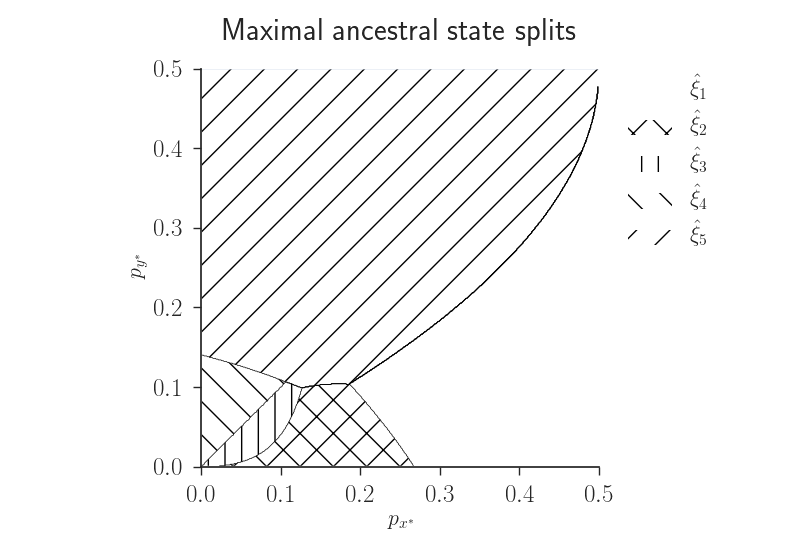
\includegraphics[width=.95\textwidth]{analytic-anc-state}
        \label{ }
    \end{minipage}
    \begin{minipage}{\linewidth}
        \centering
        Maximal ancestral state split definitions
        \begin{tabular}{l}
        \hline
        $\hat{\boldsymbol\xi}=\{\xi_{\emptyset}, \xi_{1}, \xi_{2}, \xi_{3}, \xi_{123}, \xi_{12}, \xi_{23}, \xi_{13}\}$\\
        \hline
        $\hat{\boldsymbol\xi}_1=\{\emptyset, \emptyset, \emptyset, \emptyset, \emptyset, \emptyset, \emptyset, \emptyset\}$\\
        $\hat{\boldsymbol\xi}_2=\{\emptyset, \emptyset, \emptyset, \emptyset, \{1,2\}, \emptyset, \emptyset, \emptyset\}$\\
        $\hat{\boldsymbol\xi}_3=\{\emptyset, \emptyset, \emptyset, \emptyset, \{1,2\}, \emptyset, \{1\}, \emptyset\}$\\
        $\hat{\boldsymbol\xi}_4=\{\emptyset, \emptyset, \emptyset, \emptyset, \{1,2\}, \emptyset, \{1,\}, \{1,2\}\}$\\
        $\hat{\boldsymbol\xi}_5=\{\emptyset, \emptyset, \emptyset, \{1\}, \{1\}, \emptyset, \{1\}, \{1\}\}$\\
        \hline
        \end{tabular}
    \end{minipage}
\caption{
Regions of maximal ancestral state splits on the InvFels tree $\tau_1$.
}
\label{fig:max-anc-state}
\end{figure}

Mapping each maximal ancestral state split to each likelihood value, we see that $\hat{w}\equiv 1$ if $\hat{\boldsymbol\xi}=\hat{\boldsymbol\xi}_1$ or $\hat{\boldsymbol\xi}=\hat{\boldsymbol\xi}_2$, which encompasses the bottom-right region of Figure~\ref{fig:max-anc-state}.
\end{proof}

The regions in Fig.~\ref{fig:max-anc-state} are analytically-derived regions of inconsistency in terms of probabilities of a character change along a branch for ``perfect'' data generated on the InvFels topology (Fig.~\ref{fig:farris-fels-top}) with $p_{w^*} = p_{y^*}$ (in terms of fidelities, $w^*=y^*$).
As the region of degeneracy in Fig.~\ref{fig:max-anc-state} gives the values of $x^*$ and $y^*$ where $\hat{w}$ is guaranteed to be one, we converge on a multifurcating topology in these cases.
%EM "letting $\emptyset$ be the maximal ancestral state split" sounds a little funny-- either it is or it isn't maximal.
It is easy to see that when $\emptyset$ is the maximal ancestral state split, we have the same log-likelihood for $\tau_1$ and $\tau_2$.
Moreover, if $w=1$, the internal branch becomes zero-length and the two topologies are indistinguishable.
Let $\mathcal{T}_0$ be such that, for $t^*=\{x^*,y^*,x^*,y^*,y^*\}$, $t^*\in\mathcal{T}_0$ corresponds to $x^*$ and $y^*$ falling in the region in Fig.~\ref{fig:max-anc-state} where $\hat{\boldsymbol\xi}=\hat{\boldsymbol\xi}_1$.
We can see this results in the likelihood of both topologies being equal, i.e.,
\begin{align*}
\max_{t : t^*\in\mathcal{T}_0} & \ \ell_{\tau^*,t^*}(\tau_1, t; \boldsymbol\xi)\\
&= \max_{t: \boldsymbol\xi=\hat{\boldsymbol\xi}_1, w=1, \tau=\tau_1} \ \Pr(\siteSplitRV=\siteSplit_j \mid \tau^*, t^*) \cdot \Pr(\siteSplitRV=\siteSplit_j, \ancestralSplitRV=\xi_{\siteSplit_j} \mid \tau, \{x_1,y_1,x_2,y_2,w\})\\
&= \max_{t: \boldsymbol\xi=\hat{\boldsymbol\xi}_1, w=1, \tau=\tau_2} \ \Pr(\siteSplitRV=\siteSplit_j \mid \tau^*, t^*) \cdot \Pr(\siteSplitRV=\siteSplit_j, \ancestralSplitRV=\xi_{\siteSplit_j} \mid \tau, \{x_1,y_1,x_2,y_2,w\}).
\end{align*}

%~~~
% Figures mentioned in main section of manuscript

\begin{figure}
\centering
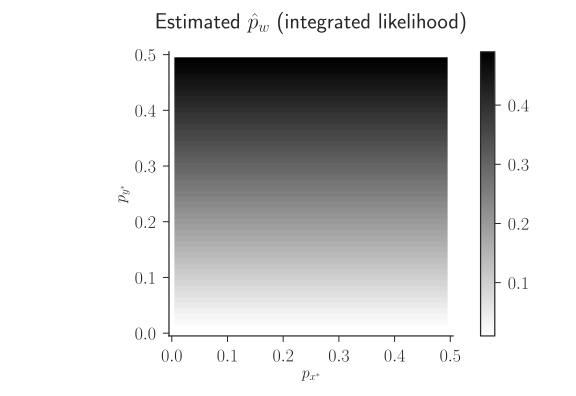
\includegraphics[width=\textwidth]{empirical-marginal}
\caption{
    Estimates for $\hat{p}_w$ when computing $(\hat{x}_1, \hat{y}_1, \hat{x}_2, \hat{y}_2, \hat{w})$ using L-BFGS-B optimizing the classical integrated likelihood \eqref{eq:marginal_likelihood} rather than a joint optimization procedure.
}
\label{fig:bl-general-marginal}
\end{figure}
%
%\begin{figure}
%\centering
%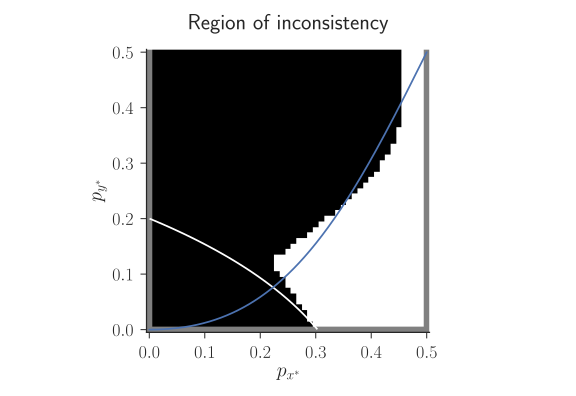
\includegraphics[width=.95\textwidth]{empirical-incons-intuition}
%\caption{
%Inconsistency in joint inference with intuitive curves.
%The white curve is our condition on the gradients.
%The blue curve is a condition on $x^*$ and $y^*$ such that $\emptyset$ is the most likely ancestral state.
%}
%\label{fig:empirical-incons-intuition}
%\end{figure}

